\section{A retention window in large driven rings}\label{sec:layer}
Consider a homogeneous $m$-state ring with one open state, rates $k_+>k_->0$,
drift $v=k_+-k_-$ in sites per unit time, and deterministic flight time $\tau$.
As $m$ increases the open fraction $1/m$ decreases. We therefore compare
$D_m(c)=[T(c)-T(0)]/m$ at fixed rates, $\tau$, and $r$.
Put $\delta=r(1-c)$ and write $p_m(t)$ for the return probability on the
ring. The corresponding return probability on the infinite lattice is
\[
 g(t)=e^{-(k_++k_-)t}I_0(2\sqrt{k_+k_-}\,t),
 \qquad H(\tau)=\int_0^\tau g(s)\,ds.
\]
Here $I_0$ is the modified Bessel function. The expression for $g$ follows
by equating independent clockwise and counterclockwise Poisson jump counts.

\paragraph{Proposition 3.}
For fixed $0<c<1$,
\[
 \lim_{m\to\infty}D_m(c)=c\int_0^\infty e^{-\delta s}g(s+\tau)\,ds>0 .
\]
At full retention, $\lim_{m\to\infty}D_m(1)=1/(2v)-H(\tau)$.
For $c_m\in[0,1]$ with $mr(1-c_m)\to z\in(0,\infty)$,
\begin{equation}
 \lim_{m\to\infty}D_m(c_m)=
 F_\tau(z)=\frac{1}{v(1-e^{-z/v})}-\frac{1}{z}-H(\tau).
 \label{eq:ring-layer}
\end{equation}
The continuous extension $F_\tau(0)$ equals the full-retention limit.
There is a unique flight time $\tau_*>0$ satisfying
$H(\tau_*)=1/(2v)$. For $\tau>\tau_*$ the limiting excess is negative at
full retention, although every fixed $0<c<1$ gives positive limiting excess.
Within the scaling in (\ref{eq:ring-layer}) there is a unique $z_*>0$
such that $F_\tau(z)<0$ for $0<z<z_*$ and $F_\tau(z)>0$ for $z>z_*$.

\paragraph{Proof.}
Equation (\ref{eq:main}) gives
$D_m(c)=c\int_0^\infty e^{-\delta s}[p_m(s+\tau)-1/m]\,ds$.
Couple the ring walk to the infinite walk reduced modulo $m$. For fixed $s$
this gives $p_m(s)\to g(s)$, hence the first limit by dominated convergence.
For the other two limits put
$B_m(\delta)=\int_0^\infty e^{-\delta t}[p_m(t)-1/m]\,dt$, including
$\delta=0$ by finite-state mixing. Then, for $c>0$,
\[
 D_m(c)/c=e^{\delta\tau}
 \left[B_m(\delta)-\int_0^\tau e^{-\delta s}[p_m(s)-1/m]\,ds\right].
\]
At $\delta=0$, $B_m(0)$ is a normalized Kemeny trace. Such traces for
driven rings and their reset-induced spectral shifts are studied in
\href{https://arxiv.org/abs/2302.09965}{Mazzolo and Monthus (2023)}.
Writing $A=k_++k_-$, the Fourier modes are
$\lambda(\theta)=-A(1-\cos\theta)+iv\sin\theta$, $\theta=2\pi j/m$.
Taking the real part gives
\[
 B_m(0)=\frac{1}{m}\sum_{j=1}^{m-1}
 \frac{A}{2[v^2+4k_+k_-\sin^2(\pi j/m)]}
 \ \longrightarrow\ \frac{1}{2v}.
\]
The last integral follows by the tangent substitution over a half period.

For $\delta>0$, set $\Delta=\sqrt{(A+\delta)^2-4k_+k_-}$ and
$u_\pm=2k_\pm/(A+\delta+\Delta)$. The infinite-line resolvent from
the origin at site $\ell\ge0$ is $u_+^\ell/\Delta$ and at $-\ell$ is
$u_-^\ell/\Delta$. Indeed these expressions solve the resolvent
recurrence $(A+\delta)G_j-k_+G_{j-1}-k_-G_{j+1}=\mathbf{1}_{\{j=0\}}$
and decay at both ends. Summing the kernel over multiples of $m$ gives
\[
 B_m(\delta)=\frac{1}{\Delta}\left[
 1+\frac{u_+^m}{1-u_+^m}+\frac{u_-^m}{1-u_-^m}\right]
 -\frac{1}{m\delta}.
\]
If $m\delta\to z>0$, then $\Delta\to v$,
$\log u_+=-\delta/v+O(\delta^2)$, and $u_-\to k_-/k_+<1$.
Substitution gives (\ref{eq:ring-layer}). The infinite-line
resolvent at the origin has limit $1/v$ as $\delta\downarrow0$, so
$H$ increases strictly from zero to $1/v$. Finally
$F_\tau'(z)=1/z^2-[4v^2\sinh^2(z/(2v))]^{-1}>0$,
and $F_\tau(+\infty)=1/v-H(\tau)>0$. These observations establish
both threshold statements. \hfill$\square$

For $k_+=1$, $k_-=0.05$, $r=0.5$, $\tau=2$, the
$m=12$ mean drops from $63.23876$ at $c=0$ to $60.57168$ at $c=1$.
The large-ring limit makes an additional prediction. For fixed $c$
below one, even a highly retentive detector eventually loses this advantage;
its mean time exceeds that for a full redraw. At the parameters above, the large-ring curve crosses zero at $z_*=5.263$, whereas the computed finite-ring crossings are $5.937$ and $5.417$ at $m=64$ and $256$, respectively. At $m=256$ the finite-ring crossing corresponds to a refresh probability $1-c=5.417/(256r)=0.0423$. This gives a control setting measurable in the original protocol. Figure~\ref{fig:layer} shows how the sign change approaches the limiting prediction.

\begin{figure}[ht]
 \centering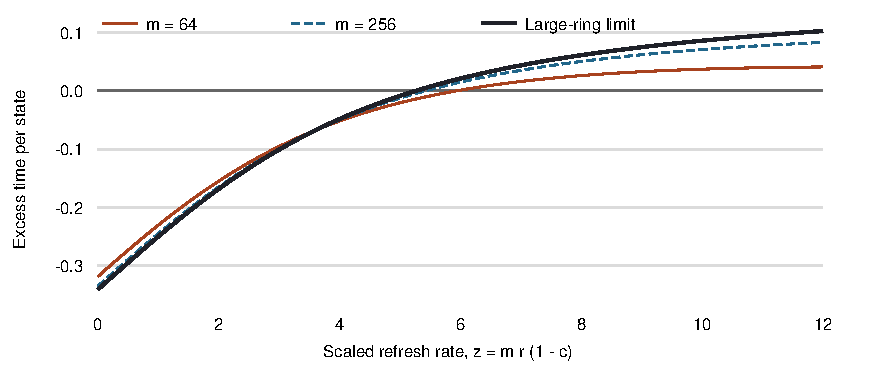
\includegraphics[width=.92\linewidth]{crossover.pdf}
 \caption{Excess mean detection time per gate state against the scaled refresh rate. Negative values favor retention relative to a full redraw. The two finite curves use the exact Fourier sum; the limiting curve uses Eq.~(\ref{eq:ring-layer}). Parameters are $k_+=1$, $k_-=0.05$, $r=0.5$, $\tau=2$.}
 \label{fig:layer}
\end{figure}
